\chapter{2$K_S^0$ invariant mass distribution}
The decay $B^0 \to K_S^0  K_S^0  K_S^0$ is much cleaner compared to the $B^0 \to K_S^+  K_S^-  K_S^0$ in terms of the $\it{CP}$-odd backgrounds, due to the absence of the \textit{u} quark in the final states. However, the potential small effect from the $\it{CP}$-odd final states mainly created by $b \to c$ transitions needs to be checked to reduce the impact on the fit of the $\it{CP}$ parameters. Usually the $\it{CP}$-odd resonant backgrounds can be effectively rejected by requiring the invariant mass of two $K_S^0$ to be outside of mass windows of the resonant intermediate states. In the early stage of the Belle II, the data validation of the two $K_S^0$ mass distribution can not be well done and such veto may contain large bias if the veto ranges are only taken from the study of MC samples. Therefore, we only present the distributions of the two $K_S^0$ invariant masses obtained from data and \textit{generic MC} in Figure \ref{fig:2ksinvm}. The contributions from $\it{CP}$-odd backgrounds will be monitored along with the future data taking.
\begin{figure}[htpb]
\begin{minipage}{0.5\linewidth}
\centering
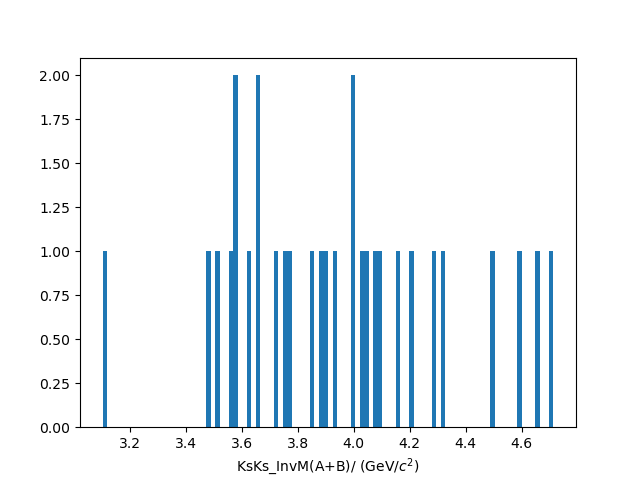
\includegraphics[width=1\linewidth]{KSKS_AB}
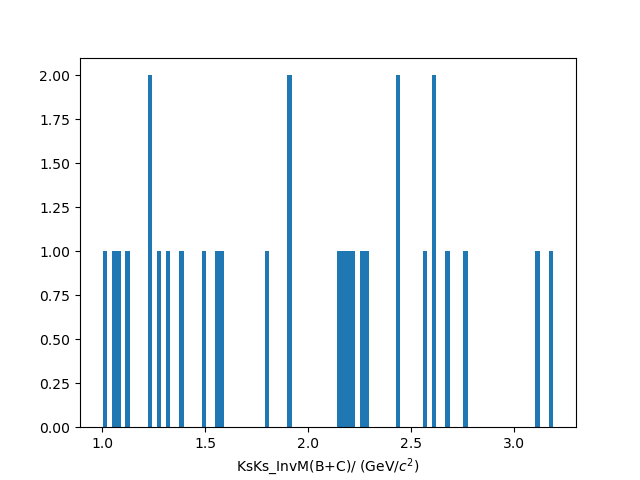
\includegraphics[width=1\linewidth]{KSKS_BC}
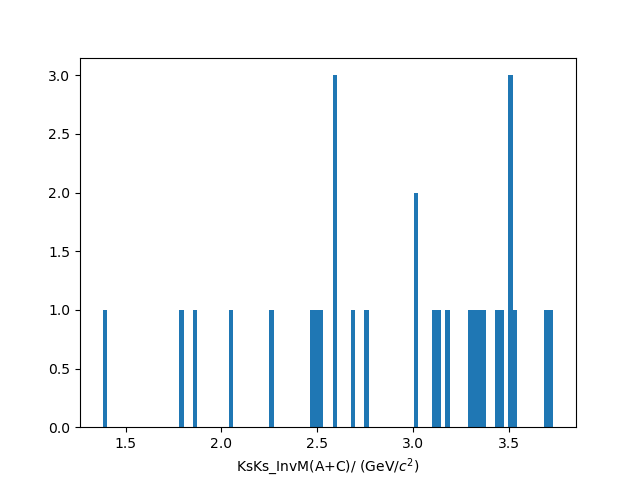
\includegraphics[width=1\linewidth]{KSKS_AC}
%\caption{The Dalitz plot in data signal region, A, B, and C is ordered according the increasing order of the momentum}
\caption{Data in signal region}
\end{minipage}
\begin{minipage}{0.5\linewidth}
\centering
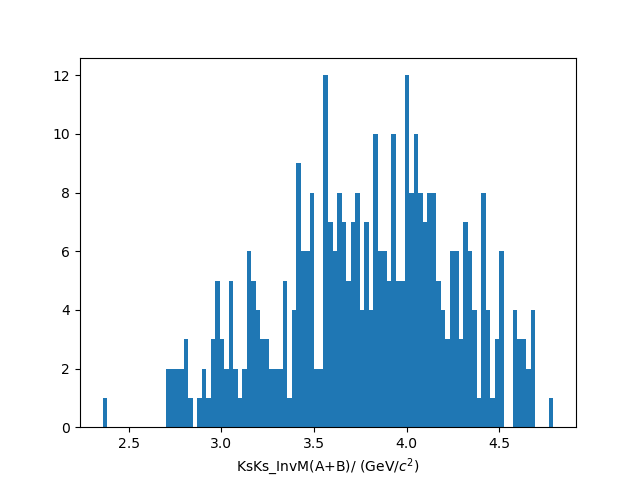
\includegraphics[width=1\linewidth]{KSKS_AB_gen}
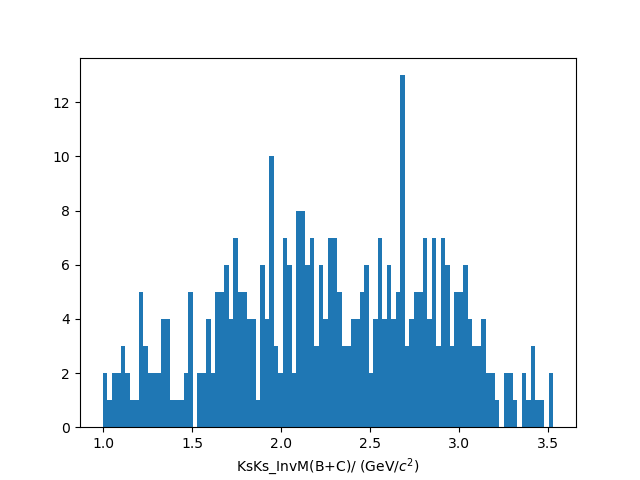
\includegraphics[width=1\linewidth]{KSKS_BC_gen}
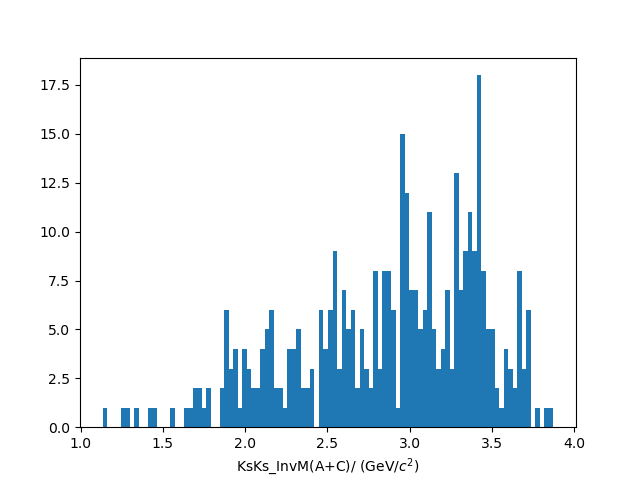
\includegraphics[width=1\linewidth]{KSKS_AC_gen}
\caption{Generic MC in signal region.}
\end{minipage}
\caption{The distribution of two $K_S^0$ invariant mass where the A, B and C indices are in the increasing order of $K_S^0$ momentum. The left is from the data and the right is from \textit{generic MC}.}
\label{fig:2ksinvm}
\end{figure}


